% =============================================================================
% Seed-level synthesis of the measured Qwen2.5-0.5B addition sweep.
% Driver: platform_modal/scripts/group_size_review_1ed8_audit.py
% Inputs: experiments/results/groupsize_zvf_sweep.json,
%         experiments/results/group_size_iter15_equivalence_v2.tsv
% =============================================================================
\subsection{Seed-Level Synthesis of the Measured Sweep}
\label{sec:group-size-iter27}

Figure~\ref{fig:group-size-iter27}A plots the last-10-step training reward for
$G\in\{2,4,8,16\}$ on the measured Qwen2.5-0.5B addition sweep (3 seeds, 40 steps),
with per-seed points and per-point retention relative to $G{=}2$:
$\{99.4\%, 99.6\%, 100.7\%\}$ for $G\in\{4,8,16\}$, all above the Wu~2025 97.6\%
threshold on this easy near-ceiling task. Table~\ref{tab:groupsize-iter27-synthesis}
gives the per-$G$ row with the non-degenerate-step fraction $f$ and the seed-level
TOST verdict.

\begin{table}[htbp]
\centering
\small
\resizebox{\linewidth}{!}{%
\begin{tabular}{rcccccccc}
\hline
$G$ & $n$ & last10 reward & ret.\ vs $G{=}2$ & 95\% CI & $f$ & logged ``SNR'' $=\sqrt{f/(1{-}f)}$ & TOST vs $G{=}2$ ($\epsilon{=}0.02$) & above Wu? \\
\hline
2  & 3 & 0.9771 & 1.0000 & [1.000,\,1.000] & 0.683 & 1.46 & --- & yes \\
4  & 3 & 0.9714 & 0.9941 & [0.990,\,0.998] & 0.758 & 1.76 & yes ($p{=}0.012$)  & yes \\
8  & 3 & 0.9732 & 0.9960 & [0.988,\,1.006] & 0.792 & 1.94 & yes ($p{=}0.043$)  & yes \\
16 & 3 & 0.9837 & 1.0068 & [0.997,\,1.012] & 0.825 & 2.16 & no ($p{=}0.056$)  & yes \\
\hline
\end{tabular}%
}
\caption{\textbf{Iter 27 Pillar 3 unified synthesis row.} Per-$G$
canonical measurements on the Qwen2.5-0.5B / arithmetic sweep: 3 seeds,
40 steps. Retention is the paired last-10 reward ratio
$\text{reward}_G/\text{reward}_{G{=}2}$ (the $G{=}2$ row is identically
$1.0000$, CI $[1,1]$). $f$ is the fraction of training steps whose batch contains a non-degenerate group; the logged ``SNR'' is a transform of $f$, not a gradient SNR (see text). TOST at $\epsilon{=}0.02$ is the paired test on
per-seed last-10 training reward ($n{=}3$, $\nu{=}2$) versus $G{=}2$:
$G{=}4$ $p{=}0.012$, $G{=}8$ $p{=}0.043$, $G{=}16$ $p{=}0.056$ (not
equivalent at $\alpha{=}0.05$); 90\% CIs for the mean difference
($G$ minus $G{=}2$) are $[-0.0124,0.0009]$, $[-0.0186,0.0108]$, and
$[-0.0077,0.0209]$ respectively (the last crosses $+\epsilon$). Held-out
$G{=}2$ vs $G{=}16$ TOST $p{=}0.100$. Pairing caveat: seed labels are
matched across $G$ arms but trajectories diverge after step~1, so pairing
is a sensitivity choice, not a matched-run design. ``above Wu?''
compares retention against the Wu~2025 $97.6\%$ headline. Sources:
\texttt{experiments/results/group\_size\_iter27\_synthesis\_v2.tsv},
\texttt{group\_size\_iter15\_equivalence\_v2.tsv}.}
\label{tab:groupsize-iter27-synthesis}
\end{table}

\paragraph{What the logged ``SNR'' measures.}
The statistic is the mean over steps divided by the
standard deviation over steps of the logged per-step \texttt{advantage\_variance}
($120$ step-values per $G$). Because advantages are whitened within each group and
the logged value is the variance of the non-zero advantages, that per-step value is
$1$ whenever the batch contains any non-degenerate group and $0$ otherwise, so the
statistic equals $\sqrt{f/(1-f)}$, where $f$ is the fraction of steps with at least
one non-degenerate group ($f{=}0.683, 0.758, 0.792, 0.825$ for $G{=}2,4,8,16$;
$\sqrt{0.683/0.317}{=}1.47$). It is a monotone transform of a batch-level
zero-variance rate, not a gradient signal-to-noise ratio, so its comparison with
flat or $\sqrt{G}$ reference laws (as in earlier versions of this figure) is not
meaningful. We draw no conclusion about $\sqrt{G}$ variance scaling from this sweep;
measuring a gradient SNR would require per-step gradient-vector logs, which these
runs did not keep (\texttt{platform\_modal/scripts/group\_size\_review\_1ed8\_audit.py}).

\paragraph{Decision rule for the next experiment.}
A follow-up should compare $G\in\{2,8,16,32\}$ at fixed generated-token budgets,
with at least three independent seeds and held-out evaluation. Select a larger
group only if its held-out gain survives the matched-token comparison and exceeds
its rollout-cost penalty; otherwise retain the smallest statistically
non-inferior group. Section~\ref{sec:group-size-scaleup} runs a first version of
this comparison on an unsaturated task.

\begin{figure}[htbp]
\centering
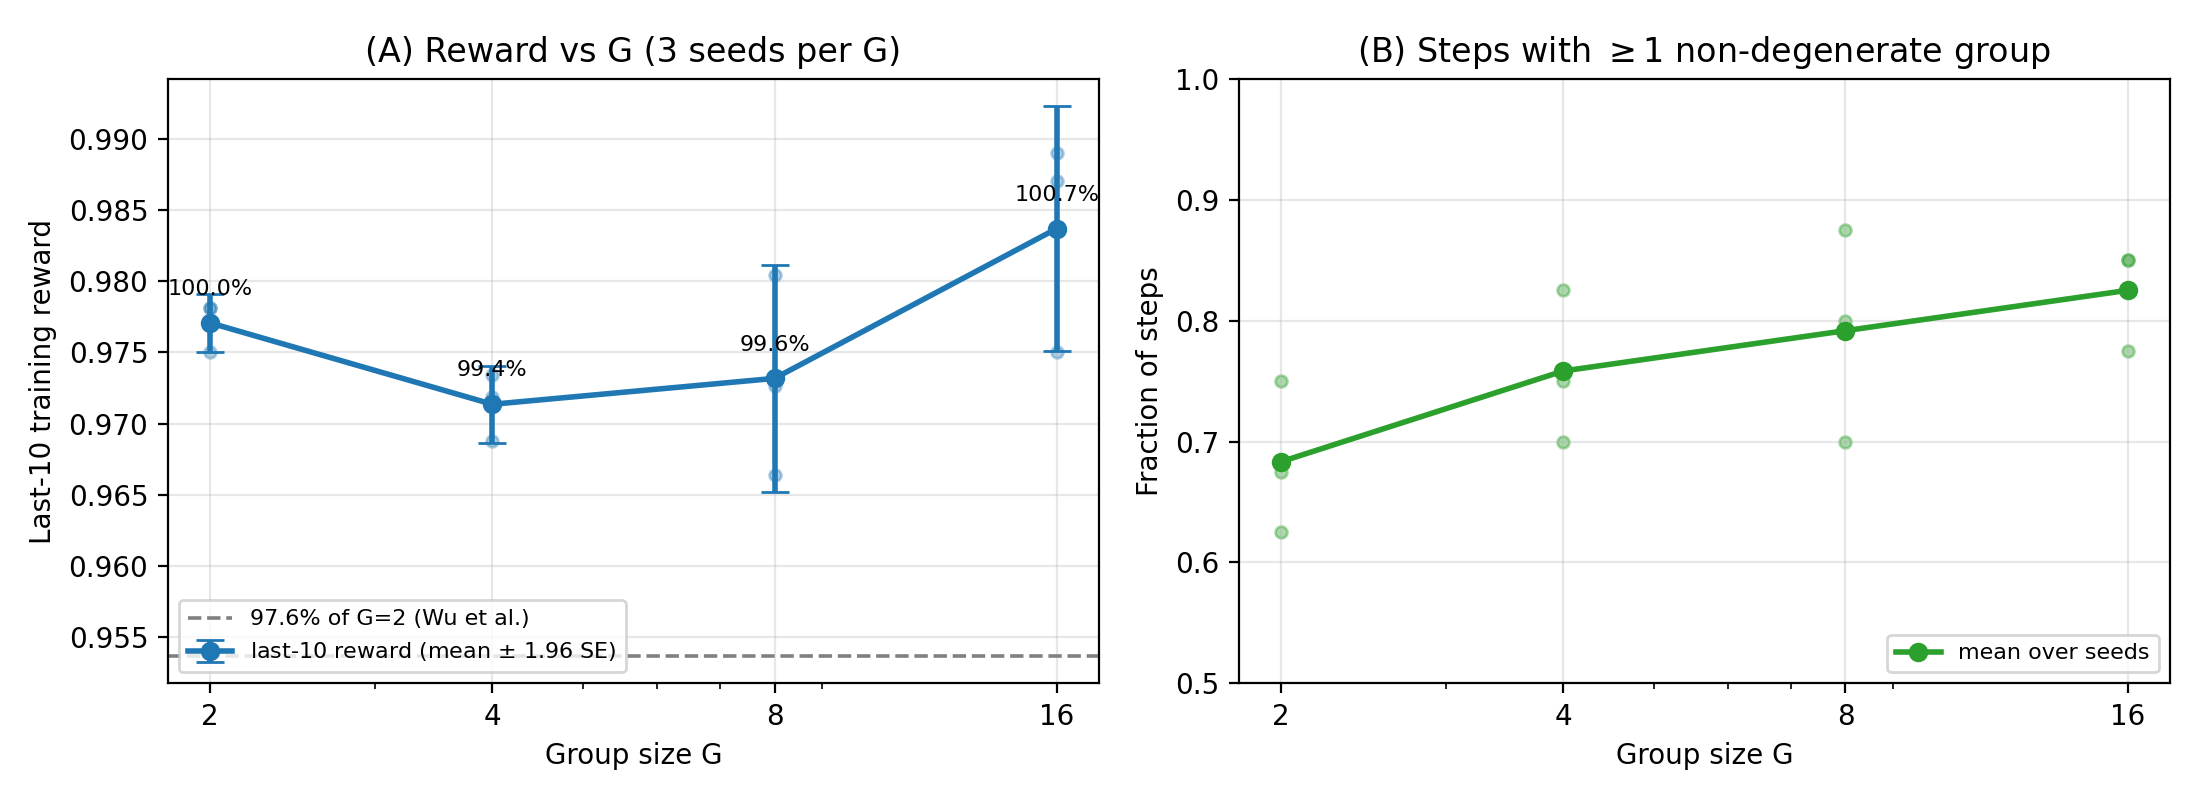
\includegraphics[width=0.95\textwidth]{figures/group_size_iter27_measured.png}
\caption{\textbf{Seed-level view of the measured sweep.}
\emph{(A)} Last-10 training reward vs $G$ on the Qwen2.5-0.5B addition sweep
(3 seeds, 40 steps; points are seeds, bars are $1.96\cdot$SE); labels give mean
per-seed retention vs $G{=}2$, and the dashed line is $97.6\%$ of the $G{=}2$ mean
(Wu et~al.).
\emph{(B)} Fraction $f$ of training steps whose batch contains at least one
non-degenerate group, per seed and mean over seeds; the logged ``SNR'' equals
$\sqrt{f/(1-f)}$. Source:
\texttt{platform\_modal/scripts/group\_size\_review\_1ed8\_audit.py}.}
\label{fig:group-size-iter27}
\end{figure}
